\documentclass[xetex,table]{beamer}

\usepackage{fontspec}
\usepackage[autostyle]{csquotes}
\usepackage{hyperref}
\usepackage{color}
\usepackage{setspace}
\usepackage{listings}
\usepackage{minted}

\usetheme{Pittsburgh}
\usecolortheme{beaver}

\title{How I survived to a SoC with a terrible Linux BSP}
\subtitle{Jurassic vendor kernels, missing pieces and buggy code}
\author{Luca Ceresoli\\
  \href{mailto:luca@lucaceresoli.net}{luca@lucaceresoli.net}\\
  \url{http://lucaceresoli.net}
}
\date{FOSDEM 2017}

\AtBeginSection[]
{
  \begin{frame}{}
    \huge
    \begin{center}
      \insertsection
    \end{center}
  \end{frame}
}

\begin{document}

\maketitle

\begin{frame}{About me}
  \begin{itemize}
  \item Open source enthusiast
    \begin{itemize}
    \item Contributor to Buildroot and a few other projects
    \end{itemize}
  \item Embedded Linux engineer
    \begin{itemize}
    \item Develop real products on custom hardware
    \item Kernel, bootloader, drivers
    \item Integration, build system
    \end{itemize}
  \end{itemize}
\end{frame}

\section{Introduction}

\begin{frame}{Typical embedded Linux system}
  \begin{itemize}
  \item A physical product
    \begin{itemize}
    \item based on an ad-hoc electronic board
    \item Built around a System-on-Chip (SoC)
    \end{itemize}
  \item Software
    \begin{itemize}
    \item Toolchain
    \item Open Source components
    \item Proprietary components
    \item A build system
    \item Board Support Package (BSP) from the SoC vendor
    \end{itemize}
  \item Most software runs equally on all SoCs (and the developer's PC)
    \begin{itemize}
    \item Except for hardware-specific code
    \end{itemize}
  \end{itemize}
\end{frame}

\begin{frame}{The System on Chip}
  \begin{itemize}
  \item Nuvoton N32926
    \begin{itemize}
    \item Cheap
    \item ARM926EJ-S @ 240 MHz
    \item Peripherals: H.264 en/decoder, Ethernet MAC, USB, CMOS
      sensor interface, video out, LCD controller, sound, \dots
    \item 64 MB DDR2 {\em on package}
    \item LQFP package
    \end{itemize}
  \item{\tiny Source:
    \url{https://www.nuvoton.com/hq/products/microprocessors/arm9-mpus/n3292-h.264-codec-series/n32926u1dn}}
  \end{itemize}
\end{frame}

\begin{frame}{The ideal BSP}
  \begin{itemize}
  \item BSP = Board Support Package
  \item The ideal BSP
    \begin{itemize}
    \item Mainline kernel
    \item Mainline U-Boot or Barebox
    \item Good hardware documentation
    \end{itemize}
  \item Why?
    \begin{itemize}
    \item All standard, open-source components
      \begin{itemize}
      \item Well known quality
      \item Community and commercial support
      \item Maintained (bugfixes!)
      \end{itemize}
    \item Reuse the infrastructure from other products
      \begin{itemize}
      \item Based on the same standard components
      \end{itemize}
    \end{itemize}
  \end{itemize}
\end{frame}

\section{The Quest}

\section{Documentation}

\begin{frame}{Public documentation}
  \begin{itemize}
  \item Website:{\tiny
    \url{https://www.nuvoton.com/hq/products/microprocessors/arm9-mpus/n3292-h.264-codec-series/n32926u1dn}}
  \item An 8-page datasheet (mostly a list of features)
  \end{itemize}
\end{frame}

\begin{frame}{Documentation for customers}
  \begin{itemize}
  \item Only under NDA
  \end{itemize}
\end{frame}

\begin{frame}{Accessible documentation}
  \begin{itemize}
  \item A ``low-cost'' devkit is available from chinese online stores
  \item Contains a DVD-ROM with a subset of the BSP for customers
    \begin{itemize}
    \item Documentation and software
    \item Contains the N3292x Design Guide
      \begin{itemize}
      \item SoC peripherals (registers)
      \end{itemize}
    \end{itemize}
  \end{itemize}
  \begin{center}
    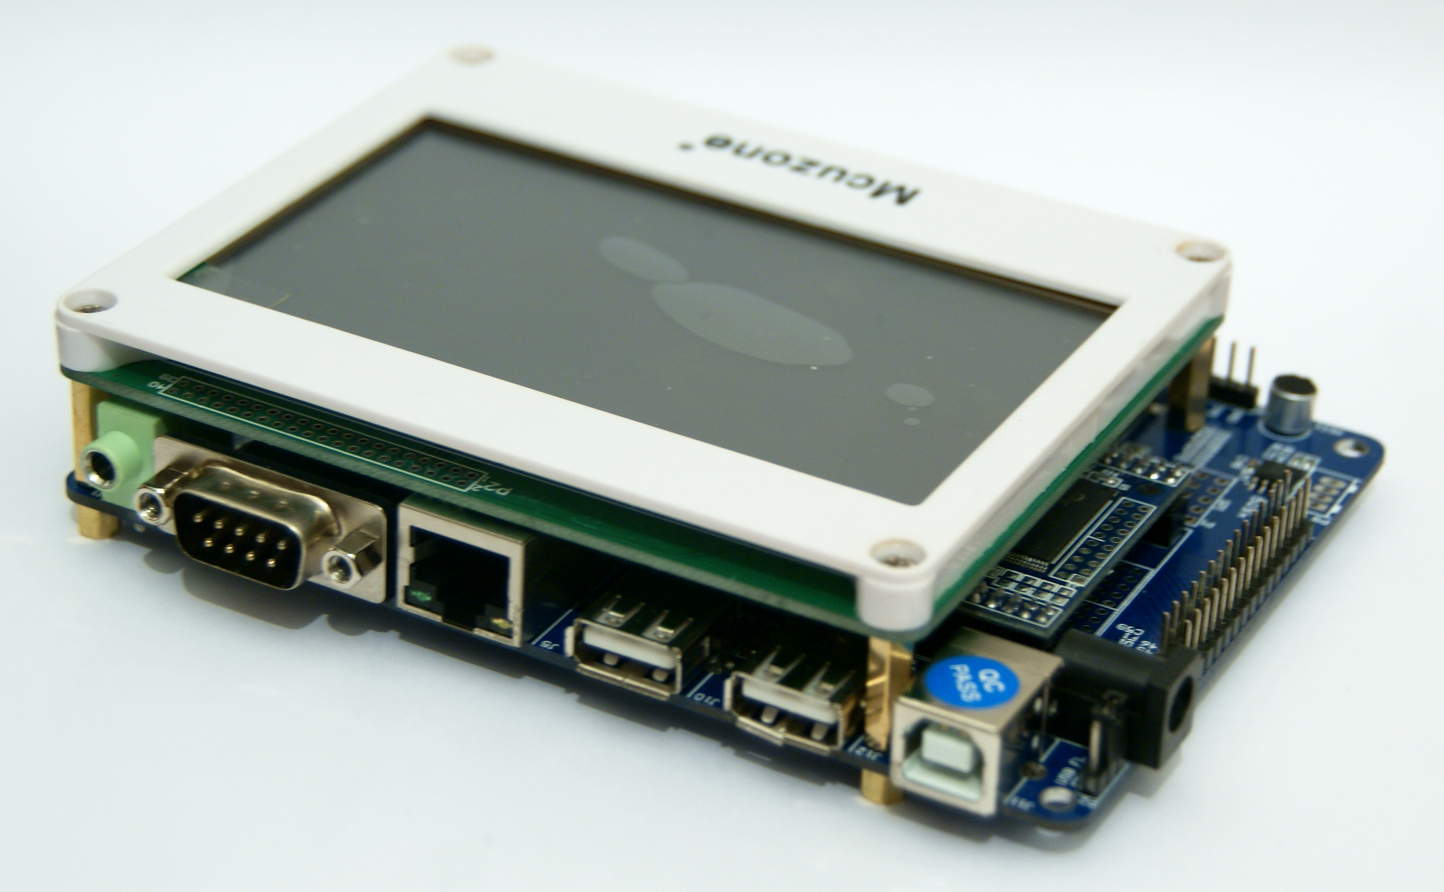
\includegraphics[height=0.4\textheight]{images/devkit.jpg}
  \end{center}
\end{frame}

\section{Linux kernel}

\begin{frame}{Vendor kernel VS mainline kernel}
  \begin{itemize}
  \item Linux 2.6.35.4 (2010)
  \item Delta from the latest 2.6.35.y (v2.6.35.14)
    \begin{itemize}
    \item 11 months, 1382 bugfix commits
    \item Merging them has minimal conflicts
    \end{itemize}
  \item Delta from the latest mainline release
    \begin{itemize}
    \item A countless number of bugfixes, performance improvements, new features
    \item Security
    \item Device Tree
    \end{itemize}
  \end{itemize}
\end{frame}

\begin{frame}{Vendor kernel additions}
  \begin{itemize}
  \item Provided as patches:
    \begin{itemize}
    \item \texttt{w55fa92-kernel-2.6.35-000.patch} (3.6 MB)
    \item \texttt{w55fa92-kernel-2.6.35-001.patch} (1.4 MB)
    \item \texttt{w55fa92-kernel-2.6.35-002.patch} (0.4 MB)
    \item \texttt{do\_kernel\_patch.sh}
    \end{itemize}
  \item Total: 170.000 lines changed
  \end{itemize}
\end{frame}

\begin{frame}{Vendor kernel issues}
  \begin{enumerate}
  \item Bugs
  \item Missing features
  \item Code quality
  \end{enumerate}
\end{frame}

\begin{frame}{Bugs}
  Examples:
  \begin{itemize}
  \item Sound Processing Unit ALSA driver
    \begin{itemize}
    \item \texttt{arecord myfile.wav} \textrightarrow{} kernel crash
      \begin{itemize}
      \item \texttt{NULL} pointer dereference
      \end{itemize}
    \end{itemize}
  \item H.264 decoder driver
    \begin{itemize}
    \item Works with sample streams
    \item Kernel crash on streaming packet loss
      \begin{itemize}
      \item Several \texttt{NULL} pointer dereferences
      \end{itemize}
    \end{itemize}
  \end{itemize}
\end{frame}

\begin{frame}{Missing features}
  Examples:
  \begin{itemize}
  \item GPIO
    \begin{itemize}
    \item Basic functionality is implemented
    \item No interrupt handling
    \end{itemize}
  \item Power Management
    \begin{itemize}
    \item Implemented with a proprietary API
    \item Also implemented the Linux standard way, but incomplete and
      not working
    \end{itemize}
  \end{itemize}
\end{frame}

\begin{frame}{Code quality}
  \begin{itemize}
  \item Average quality of additions: generally bad
  \item Trivial metric: +521 lines starting with \texttt{\#if 0}
  \item A few examples follow
  \end{itemize}
\end{frame}

\begin{frame}[fragile]{Code quality /1}
  Changes to \texttt{Makefile}:

  \begin{minted}[fontsize=\scriptsize]{diff}
-ARCH?= $(SUBARCH)
-CROSS_COMPILE?=
-CROSS_COMPILE?= $(CONFIG_CROSS_COMPILE:''%''=%)
+#ARCH?= $(SUBARCH)
+ARCH= arm
+#CROSS_COMPILE?=
+#CROSS_COMPILE?= $(CONFIG_CROSS_COMPILE:''%''=%)
+CROSS_COMPILE= arm-linux-
  \end{minted}

  \begin{itemize}
  \item Prevents using toolchains with a different prefix
  \item Any advantage?
  \end{itemize}
\end{frame}

\begin{frame}[fragile]{Code quality /2}
  Changes to \texttt{arch/arm/boot/Makefile}:

  \begin{minted}[fontsize=\scriptsize]{udiff}
 $(obj)/Image: vmlinux FORCE
         $(call if_changed,objcopy)
         @echo '  Kernel: $@ is ready'

+ifeq ($(CONFIG_ARCH_W55FA92),y)
+        cp $@   ../image/conprog.bin
+endif
  \end{minted}

  \begin{itemize}
  \item \texttt{../image/} does not make sense in any buildsystem
  \end{itemize}
\end{frame}

\begin{frame}[fragile]{Code quality /3}
  \texttt{sound/soc/w55fa92/w55fa92\_spu.c}:

  \begin{minted}[fontsize=\scriptsize]{c}
    if (nChannels ==1)
    {
        DrvSPU_EnableInt(_u8Channel0, DRVSPU_ENDADDRESS_INT);
        DrvSPU_EnableInt(_u8Channel0, DRVSPU_THADDRESS_INT);
    }
    else
    {    /* just open one channel interrupt */
        DrvSPU_EnableInt(_u8Channel0, DRVSPU_ENDADDRESS_INT);
        DrvSPU_EnableInt(_u8Channel0, DRVSPU_THADDRESS_INT);
    }
  \end{minted}

  \begin{itemize}
  \item Find the differences between the {\em then} and the {\em else} branch
  \end{itemize}
\end{frame}

\begin{frame}[fragile]{Code quality /4}
  \texttt{sound/soc/w55fa92/w55fa92\_spu.c}:

  \begin{minted}[fontsize=\scriptsize]{c}
static int DrvSPU_EnableInt(u32 u32Channel, u32 u32InterruptFlag)
{
  if ( (u32Channel >=eDRVSPU_CHANNEL_0) && (u32Channel <=eDRVSPU_CHANNEL_31) )
  {
    /* ... */
    if (u32InterruptFlag & DRVSPU_USER_INT)
    {
      AUDIO_WRITE(REG_SPU_CH_EVENT, AUDIO_READ(REG_SPU_CH_EVENT) | EV_USR_EN);
    }
    if (u32InterruptFlag & DRVSPU_SILENT_INT)
    {
      AUDIO_WRITE(REG_SPU_CH_EVENT, AUDIO_READ(REG_SPU_CH_EVENT) | EV_SLN_EN);
    }
    /* ...a few more times... */

    /* ... */
    return E_SUCCESS;
  }
  else
    return E_DRVSPU_WRONG_CHANNEL;
}
  \end{minted}
\end{frame}

\begin{frame}[fragile]{Code quality /5}
  \texttt{arch/arm/mach-w55fa92/include/mach/w55fa92\_gpio.h}:

  \begin{minted}[fontsize=\scriptsize]{c}
static inline int w55fa92_gpio_configure(int group, int num) {
  /* ... */
    case GPIO_GROUP_B:
      if(num <= 7)
        writel(readl(REG_GPBFUN0) &~ (0xF << (num<<2)), REG_GPBFUN0);
      else
        writel(readl(REG_GPBFUN1) &~ (0xF << ((num%8)<<2)), REG_GPBFUN1);
      break;

    case GPIO_GROUP_C:
      if(num <= 7)
        writel(readl(REG_GPCFUN0) &~ (0xF << (num<<2)), REG_GPCFUN0);
      else
        writel(readl(REG_GPCFUN1) &~ (0xF << ((num%8)<<2)), REG_GPCFUN1);
      break;
  /* ...similarly fo other GPIO ports... */
}
  \end{minted}

  \begin{itemize}
  \item A little refactoring would help
  \end{itemize}
\end{frame}

\begin{frame}[fragile]{Code quality: driver model}
  \texttt{drivers/video/w55fa92\_fb.c}:

  \begin{minted}[fontsize=\scriptsize]{c}
#ifdef  CONFIG_GIANTPLUS_GPM1006D0_320X240
#include "w55fa92_GIANTPLUS_GPM1006D0.c"
#endif

#ifdef  CONFIG_TOPPLY_320X240
#include "w55fa92_TOPPLY_320x240.c"
#endif

/* ...5 more displays... */

#if 0
  #ifdef  CONFIG_SHARP_LQ035Q1DH02_320X240
  #include "w55fa92_Sharp_LQ035Q1DH02.c"
  #endif

  #ifdef  CONFIG_WINTEK_WMF3324_320X240
  #include "w55fa92_Wintek_WMF3324.c"
  #endif

  /* ...5 more displays... */
#endif
  \end{minted}
\end{frame}

\begin{frame}[fragile]{Code quality: H.264 codec memory allocation}
  \texttt{drivers/misc/codec264/favc\_module.c}:

  \begin{minted}[fontsize=\scriptsize]{c}
unsigned int get_avc_buffer_size(void)
{
  /* ...~90 lines... */
  return TOTAL_VDE_BUF_SIZE;
}
EXPORT_SYMBOL(get_avc_buffer_size);
  \end{minted}

  From {\small\texttt{arch/arm/mm/mmu.c}}:
  \begin{minted}[fontsize=\scriptsize]{c}
extern unsigned int get_avc_buffer_size(void);
void __init reserve_node_zero(pg_data_t *pgdat)
{
  /* ... */
  buffer_size = get_avc_buffer_size();
  printk("AVC Buffer Size: 0x%x\n",buffer_size);
  w55fa92_vde_v = alloc_bootmem_low_pages (buffer_size);
  /* ... */
}
  \end{minted}
\end{frame}

\section{Concluding remarks}

\begin{frame}
  \begin{center}
    Thank you for your attention

    \vspace{0.15\textheight}

    {\Huge Questions?}

    \vspace{0.15\textheight}

    \href{mailto:luca@lucaceresoli.net}{luca@lucaceresoli.net}\\
    \url{http://lucaceresoli.net}

    \textcopyright{} Copyright 2017, Luca Ceresoli\\

    \vspace{0.05\textheight}

    \tiny
    Slides released under\\
    Creative Commons Attribution - Share Alike 3.0 License \\
    \url{https://creativecommons.org/licenses/by-sa/3.0/} \\
\end{center}
\end{frame}

\end{document}
